% Workflow regression for the trees library three-point growth function.
\documentclass[border=2pt]{standalone}
\usepackage{tikz}
\usetikzlibrary{trees}

\tikzset{
  stage/.style={draw,rounded corners=2pt,minimum width=18mm,minimum height=8mm,inner sep=2pt},
  every edge from parent/.style={draw,thick,-stealth}
}

\begin{document}
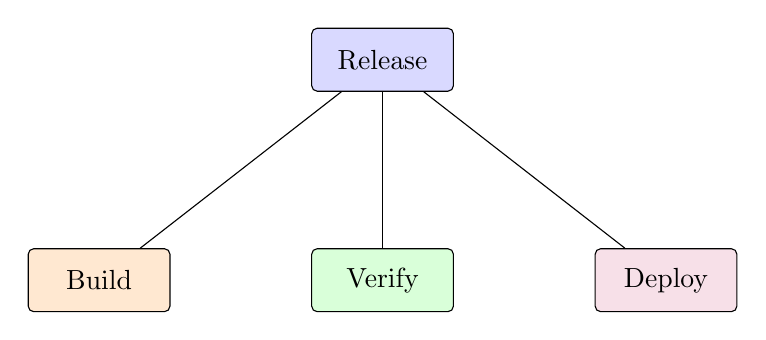
\begin{tikzpicture}[
  level 1/.style={grow via three points={one child at (0,-12mm) and
    two children at (-18mm,-20mm) and (18mm,-20mm)}}
]
  \node[stage,fill=blue!15] {Release}
    child {node[stage,fill=orange!18] {Build}}
    child {node[stage,fill=green!15] {Verify}}
    child {node[stage,fill=purple!12] {Deploy}};
\end{tikzpicture}
\end{document}
